%(BEGIN_QUESTION)
% Copyright 2009, Tony R. Kuphaldt, released under the Creative Commons Attribution License (v 1.0)
% This means you may do almost anything with this work of mine, so long as you give me proper credit

Read and outline the ``Dual-Beam Analyzer'' subsection of the ``Non-Dispersive Luft Detector Spectroscopy'' section of the ``Continuous Analytical Measurement'' chapter in your {\it Lessons In Industrial Instrumentation} textbook.  Note the page numbers where important illustrations, photographs, equations, tables, and other relevant details are found.  Prepare to thoughtfully discuss with your instructor and classmates the concepts and examples explored in this reading.

\underbar{file i04168}
%(END_QUESTION)




%(BEGIN_ANSWER)


%(END_ANSWER)





%(BEGIN_NOTES)

A dual-beam NDIR analyzer splits the source light beam into two halves, passing it through two identical chambers.  One chamber is filled with a non-absorbing ``reference'' gas, while the other chamber is filled with sample gas to be analyzed.  A pair of series-opposed thermopiles compares the optical output of the two chambers, outputting the difference between the two.

\vskip 10pt

This design completely eliminates the ambient temperature drift problem, and it also eliminates zero drift due to changes in source light intensity.  Span drift still occurs if the source light becomes brighter or dimmer, and the analyzer is still completely non-selective.

\vskip 10pt

One improvement to combat errors to due mismatches between the two thermopiles is to ``chop'' the light beam, then demodulate the thermopile signals.  Any mismatch or thermal drift between the two detectors will manifest as a DC offset voltage, while any signal caused by the presence of light-absorbing gas in the sample cell will manifest as an AC (pulse) voltage.  After de-modulation, the only signal left is that created by sample gas.





\vskip 20pt \vbox{\hrule \hbox{\strut \vrule{} {\bf Suggestions for Socratic discussion} \vrule} \hrule}

\begin{itemize}
\item{} {\bf In what ways may a dual-beam NDIR instrument be ``fooled'' to report a false composition measurement?}
\item{} Referring to a chopperless dual-beam analyzer illustration, what is the polarity of the DC signal voltage output by the two series thermopiles caused by the presences of a light-absorbing gas in the sample cell?
\item{} Referring to a chopperless dual-beam analyzer illustration, what would happen if the light source intensity were to increase/decrease?
\item{} Referring to a chopperless dual-beam analyzer illustration, what would happen if the reference chamber were to be accidently filled with light-absorbing gas?
\item{} Explain how the chopper wheel solves the problem of drift due to imbalances between the two thermopiles.
\item{} Referring to a chopper-wheel dual-beam analyzer illustration, what would happen if the light source intensity were to increase/decrease?
\item{} Referring to a chopper-wheel dual-beam analyzer illustration, what would happen if the reference chamber were to be accidently filled with light-absorbing gas?
\item{} What would happen if the sample cell's windows were to become dirty due to poorly-filtered process gas?  Would the presence of a chopper wheel improve things here?
\end{itemize}






\vfil \eject

\noindent
{\bf Prep Quiz:}

Explain why this two-beam NDIR analyzer design is superior to a single-beam NDIR analyzer design:

$$\includegraphics[width=15.5cm]{i04168x01.eps}$$

%INDEX% Reading assignment: Lessons In Industrial Instrumentation, Analytical (nondispersive spectroscopy)

%(END_NOTES)


